\chapter{CA-Stream: Attention-based pooling for interpretable image recognition}
\chaptertoc{}
\label{ch:castream}
\section{Introduction}
\label{sec:intro}
%--------------------------------------------------------------------------------------------------
\noindent Another way to approach interpretability can be pointed towards the current advances in recognition 
in general. In particular, with the introduction of the transformer architecture (\cite{vaswani2017attention})
 a switch in the paradigmn occurred where the best performing architectures contain the self-attention 
module as a building block. Moreover with the proposal of the Vision Transformer 
(\cite{dosovitskiy2020image}) transformers were adopted into computer vision, this module gained 
prominence as it allowed models to push the boundaries in existing benchmarks. This led to an 
expansion with models such as Swin-T (\cite{liu2021swin}), LeViT \cite{graham2021levit}. Conversely
hybrid architectures combining ideas from both \gls{cnn} and transformers can be observed 
like Conformer (\cite{peng2021conformer}), Patchconvnet (\cite{touvron2021augmenting}),
while on another hand a modernization of CNNs in the shape of ConvNeXt (\cite{liu2022convnet}) drew 
inspiration from these models, whilst adressing their shortcomings in downstream tasks.\\

\noindent Although these models have pushed visual recognition to new frontiers, their interpretable
 properties still require further exploration, as in one hand conventional interpretability 
methodologies for CNNs do not translate properly into their domain, all the while the explanations 
obtained from these methods (\cite{abnar2020quantifying}) do not appear to have a proper evaluation 
protocol, resulting in research aimed at improved visualizations and their asssesment 
(\cite{chefer2021transformer}).

\noindent In this chapter we study the correlation between CAM and one such attention visualization 
proposal that is the raw attention found in the classification (\cls) token (\cite{devlin2018bert}).
In particular, we note that self attention is defined for all patch tokens including \cls, however 
we can generate cross attention between this token and the feature maps found at any given depth 
of a CNN; this being expressed in via linear combination of feature maps with this token, ultimately 
resembling a class agnostic CAM. As an extension of this, we propose the inclusion of a 
cross-attention module used to train this token as a replacement of GAP (\cite{lin2013network}), 
onto already trained models boosting  both their recognition and interpretable properties.


%    \chapter*{Introduction}
    \chaptertoc{}

    \addcontentsline{toc}{chapter}{Introduction}
    \section*{Motivation}
    %\addcontentsline{toc}{section}{Motivation}

    \section*{Dissertation Outline}
    %\addcontentsline{toc}{section}{Dissertation Outline}
    This dissertation is organized in the following manner: First
    we introduce a background on existing approaches towards interpretability of image
    recognition models; for that, we make mention on current architectures dedicated 
    to this approach, while also presenting concepts on interpretability and enunciating 
    current approaches for this study. 

    In Chapter \ref{ch:opticam}, we propose Opti-CAM as a methodology that generates 
    optimized saliency maps highlighting the relevant regions on an image towards image
    classification. On Section \ref{sec:av_gain} we extend existing evaluation metrics 
    with a novel measurement for model coinfidence. extends evaluation metrics with the 
    introduction of a novel measurement yielding improvements on model confidence 
    when using a given attribution approach. On Sections \ref{sec:oc_qual, sec:oc_quant} 
    we evaluate the effect of these contributions towards interpretability assessment.
    
    Chapter \ref{ch:castream} introduces the Cross Attention Stream, an approach that boosts
     existing architectures interpretable properties. We ste up the modulus of this approach 
    on Section \ref{sec:ca_defn} alongside its deployment on Section \ref{sec:ca_design}. 
    On Sections \ref{sec:ca_qual} and \ref{sec:ca_quant} we demonstrate the benefits 
    of using this proposal.
    
    Chapter \ref{ch:grad} characterizes a gradient denoising approch with a gradient denoising
     methodology as an approach to enhance the trainining procedure of current
    models while improving interpretability properties. On Section \ref{sec:grad_defn}, 
    we define the gradient denoising protocol alongside the regularization proposals to do so.
    Sections \ref{sec:grad_qual, sec:grad_quant} illustrate the effects of this paradigmn
    on the trained models and its effects on interpretability.
    
    Chapter \ref{ch:zip} raises the Zero-Information algorithm and its usage as a substitute
    for mask-dependent evaluation proposals. Section \ref{sec:zip_algo} develops this 
    method. Section \ref{sec:zip_insdel} demonstrates its incorporation of this 
    algorithm onto evaluation protocols. Section \ref{sec:zip_qual} displays
    the effect of this approach when applied to mask patches on images. Section 
    \ref{sec:zip_benchmark} displays the results of benchmarking these protocols 
    with this approach. 
    
    Finally, 
    we draw conclusions on our work and detail future research perspectives.


\section {Cross Attention}
\label{sec:ca_defn}
%--------------------------------------------------------------------------------------------------
%\paragraph{Cross attention}
Let matrix $F_\ell \in \real^{p_\ell \times d_\ell}$ be a reshaping of feature tensor $\vF_\ell$ at
 layer $\ell$, where $p_\ell \defn w_\ell h_\ell$ is the number of patch tokens without \cls, and
  let $\vq_\ell \in \real^{d_\ell}$ be the \cls token embedding at layer $\ell$. By focusing on the 
  \emph{cross attention} only between the \cls (query) token $\vq_\ell$ and the patch (key) tokens 
  $F_\ell$ and by ignoring projections $W_Q, W_K, W_V$ for simplicity, attention $A$~\eq{attention} 
  is now a $1 \times p_\ell$ matrix that can be written as a vector $\mathbf{a} \in \real^{p_\ell}$

\begin{equation}
	\mathbf{a} = A\tran = \softmax \left( \frac{F_\ell \vq_\ell}{\sqrt{d_\ell}} \right).
\label{eq:cross-attention}
\end{equation}

Here, $F_\ell \vq_\ell$ expresses the pairwise similarities between the global \cls feature 
$\vq_\ell$ and the local patch features $F_\ell$. Now, by replacing $\vq_\ell$ by an arbitrary vector 
$\mathbf{a}lpha \in \real^{d_\ell}$ and by writing the feature matrix as $F_\ell = (\vf_\ell^1 \dots 
\vf_\ell^{d_\ell})$ where $\vf_\ell^k = \vect(F_\ell^k) \in \real^{p_\ell}$ for channel $k$, 
attention \eq{cross-attention} becomes

\begin{equation}
	\mathbf{a} = h_\ell (F_\ell \mathbf{a}lpha) =
		h_\ell \left( \sum_k \alpha_k \vf_\ell^k \right).
\label{eq:connection}
\end{equation}
This takes the same form as~\eq{sal}, with feature maps $F_\ell^k$ being vectorized into 
$\vf_\ell^k$ and the activation function is defined as $h_\ell(\vx) = \softmax(\vx / \sqrt{d_\ell})$. 
Eq.~\eq{connection} is visualized in \autoref{fig:connection}. We thus observe the following.

\begin{quote}
	\emph{Pairwise similarities between one query and all patch token embeddings in cross attention 
	are the same as a linear combination of feature maps in CAM-based saliency maps, where the 
	weights are determined by the elements of the query.}
\end{quote}

As it stands, one difference between~\eq{sal} and~\eq{connection} is that~\eq{connection} is class 
agnostic, although it could be extended by using one query (weight) vector per class. For simplicity, 
we choose the class agnostic form in the following. %We also choose to have no query/key projections. 
%However, we do provide additional experiments with class specific representation as well as projections in \autoref{sec:gen_ablation}. 

%--------------------------------------------------------------------------------------------------
\paragraph{Pooling, or masking}

We are thus motivated to integrate an attention mechanism into any network such that making a 
prediction and explaining (localizing) it are inherently connected. In particular, considering 
cross attention only between \cls and patch tokens~\eq{cross-attention}, equation~\eq{SA} becomes

\begin{align}
	\ca_\ell(\vq_\ell, F_\ell) \defn F_\ell\tran \mathbf{a} = F_\ell\tran h_\ell(F_\ell \vq_\ell) 
	\in \real^{d_\ell}.
\label{eq:CA}
\end{align}

By writing the transpose of feature matrix as $F_\ell\tran = (\vphi_\ell^1 \dots 
\vphi_\ell^{p_\ell})$ where $\vphi_\ell^i \in \real^{d_\ell}$ is the feature of patch $i$, 
this is a weighted average of the local patch features $F_\ell\tran$ with attention vector 
$\mathbf{a} = (a_1, \dots, a_{p_\ell})$ expressing the weights:

\begin{align}
	\ca_\ell(\vq_\ell, F_\ell) \defn F_\ell\tran \mathbf{a} = \sum_i a_i \vphi_\ell^i.
\label{eq:CA-gap}
\end{align}
We can think of it as as feature \emph{reweighting} or \emph{soft masking} in the feature space, 
followed by \gap.

Now, considering that $\mathbf{a}$ is obtained exactly as CAM-based saliency maps~\eq{connection}, 
this operation is similar to occlusion (masking)-based methods \autocite{petsiuk2018rise, 
fong2017interpretable, fong2019understanding, schulz2020restricting, ribeiro2016should,
wang2020score, zhang2023opti} and evaluation metrics \autocite{chattopadhay2018grad, 
petsiuk2018rise}, where a CAM-based saliency map is commonly used to mask the input image. 
We thus observe the following.

\begin{quote}
	\emph{Attention-based pooling is a form of feature reweighting or soft masking in the feature 
	space followed by \gap, where the weights are given by a class agnostic CAM-based saliency map.}
\end{quote}

%\begin{figure}[t]
    \centering
    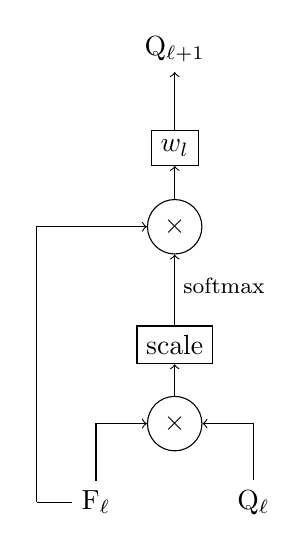
\begin{tikzpicture}
        \node (Q) at (4.5, -0.5) {Q$_\ell$};
        % \node (dimq) at (5, 0) {\scriptsize${1\times d_\ell}$};
        \node (F) at (2.5, -0.5) {F$_{\ell}$};
        % \node (dimft) at (3.0, -0) {\scriptsize${d_{\ell}\times p}$};
        \node (empt1) at (1.75, -0.5) {};
        \node[shape=circle,draw=black] (mm1) at (3.5, 0.5) {$\times$};
        % \node (dimraw) at (4,1) {\scriptsize$1\times p$};
        \node[shape=rectangle,draw=black](scale) at (3.5, 1.5) {scale};
        % \node (dimf) at (2.5, 3.175) {\scriptsize${p\times d_{\ell}}$};
        \node (soft) at (4.125, 2.25) {\footnotesize softmax};
        \node[shape=circle,draw=black] (mm2) at (3.5, 3) {$\times$};
        % \node[shape=rectangle,draw=black](project) at (3.5, 4) {$w_l: d_\ell\times d_{\ell+1}$ };
        \node[shape=rectangle,draw=black](project) at (3.5, 4) {$w_l$};
        % \node (dimscaled) [] at (4.25, 3.5) {\scriptsize $1\times d_\ell$};
        % \node [shape=circle,draw=black](sum1) at (3.5, 4) {+};
        % \node [shape=rectangle,draw=black](norm) at (3.5, 5.75) {LayerNorm};
        \node (Qplus1) at (3.5, 5.25) {Q$_{\ell+1}$};
        % \node (dimql) [align=left] at (4.25, 4.75) {\scriptsize$1\times d_{\ell+1}$};
        % \node (empt2) at (5.75, -0.5) {};

        \draw[->] (Q) |- node {} (mm1);
        \draw[->] (F) |- node {} (mm1);
        % \draw[-] (Q) -| node {} (empt2);
        % \draw[->] (empt2.center) |- node {} (sum1);
        \draw[->] (mm1) -- node {} (scale);
        \draw[->] (scale) -- node {} (mm2);
        \draw[-] (F) -| node {} (empt1.center);
        \draw[->] (empt1.center) |- node {} (mm2);
        \draw[->] (mm2) -- node {} (project);
        % \draw[->] (sum1) -- node {} (project);
        \draw[->] (project) -- node {} (Qplus1);
        % \draw[->] (norm) -- node {} (Qplus1);
    \end{tikzpicture}
    \caption{A Cross Attention Block. We denote matrix multiplication as "$\otimes$". The softmax operation is performed on each row). For a given layer $\ell$ we update our [CLS] token $Q_\ell$; by computing its scaled cross attention with the feature maps $F_\ell$, that are then projected to the channel dimension in the following stage, using a dense layer parametrized by $w_\ell$.}
    \label{fig:fig_crossatt}
\end{figure}

\section{Cross Attention Stream}
\label{sec:ca_design}
\input{fig/castream/ca_mainfig.tex}
\section{Experiments}
\label{sec:exp}

We evaluate the interpretability and recognition capabilities of our approach. In particular, we generate explanations following current state-of-the art post-hoc interpretability methods derived from CAM~\cite{zhou2016learning}. We compare the properties of the backbone network $f$ with and without our \Ours, where $f$ is pretrained and fixed.

\subsection{Experimental setup}
\label{subsec:setup}

\paragraph{Training}

We train and evaluate our models on the ImageNet ILSVRC-2012 dataset~\cite{deng2009imagenet}, on the training and validation splits respectively. Thus, we experiment with ResNet-based architectures~\cite{he2016deep} such as ResNet-18 and ResNet-50, and ConvNeXt based architectures~\cite{liu2022convnet} such as ConvNeXt-Small and ConvNeXt-Base. We aim at learning our \Ours, generating a \cls token that interacts with feature maps at different stages of network $f$, to serve as an attention-based pooling mechanism in order to interpret the predictions of $f$. Therefore, we experiment with pretrained models\footnote{https://pytorch.org/vision/0.8/models.html}, that we keep frozen while the parameters of the \Ours are optimized. Details on training hyperparameters are given in the appendix.

Moreover, we present experiments on the bird dataset: CUB-200-2011 \cite{WahCUB_200_2011} and on PASCAL VOC 2012 dataset \cite{Everingham15}. Here the ResNet-50 network is fine-tuned to these dataset as baseline. Then, our \Ours is learned as for ImageNet.

\paragraph{Evaluation}

We employ existing post-hoc interpretability methods to generate saliency maps with and without \Ours and compare interpretability metrics as well as classification accuracy. Regarding interpretability methods, we use Grad-CAM~\cite{DBLP:journals/corr/SelvarajuDVCPB16}, Grad-CAM++~\cite{DBLP:journals/corr/abs-1710-11063} and ScoreCAM~\cite{DBLP:journals/corr/abs-1910-01279}. We note that the evaluation is performed on the entire validation set, unlike the previous approaches.

Following Opti-CAM~\cite{zhang2023opti}, we use a number of classification metrics for interpretability. In particular, we consider the changes in predictive power measured by \emph{average drop} (AD)~\cite{DBLP:journals/corr/abs-1710-11063} and \emph{average gain} (AG)~\cite{zhang2023opti}, the proportion of better explanations measured by \emph{average increase} (AI)~\cite{DBLP:journals/corr/abs-1710-11063} and the impact of different extent of masking measured by \emph{insertion} (I) and \emph{deletion} (D)~\citep{petsiuk2018rise}.

% For localization, we use metrics from the \emph{weakly-supervised object localization} (WSOL) task to measure the maximum overlap between the saliency map (or corresponding predicted bounding boxes) and ground truth bounding boxes, \ie \emph{official metric} (OM), \emph{localization error} (LE), \emph{pixel-wise $F_1$ score}, \emph{box accuracy} (BoxAcc)~\citep{choe2020evaluating} and \emph{saliency metric} (SM)~\citep{dabkowski2017real}. We also measure the localization of the pixel of maximum saliency by the \emph{standard pointing game} (SP)~\cite{zhang2018top} and the fraction of the saliency map within the ground truth bounding boxes by \emph{energy pointing game} (EP)~\citep{DBLP:journals/corr/abs-1910-01279}. We obtain the ground truth bounding boxes from the ILSVRC2014\footnote{\url{https://www.image-net.org/challenges/LSVRC/2014/index\#}} dataset. 



%--------------------------------------------------------------------------------------------------
\section{Qualitative Results}
\label{sec:ca_qual}
\subsection{Qualitative evaluation}
\label{subsec:vinspection}    
We show saliency maps obtained by different interpretability methods using either \gap or \Ours, as 
well as the class-agnostic raw attention coming from our \Ours, see \autoref{fig:compmethods}.\\
%--------------------------------------------------------------------------------------------------
\begin{figure}[H]
    \scriptsize
    \centering
    \setlength{\tabcolsep}{1.5pt}
    % \resizebox{\textwidth}{!}{%
    \begin{tabular}{ccccccccc}
        {}&\multirow{2}{*}{Input image}&\multirow{2}{*}{Raw Attention}&\multicolumn{2}{c}{Grad-CAM}&\multicolumn{2}{c}{Grad-CAM++}&\multicolumn{1}{c}{Score-CAM}\\
        {}&{}&{}&GAP&\Ours&GAP&\Ours&GAP&\Ours\\   
        {\rotatebox{90}{\tiny Envelope}}&\includegraphics[width=0.115\textwidth]{fig/castream/images/Comparable/figure1_similarities/original/23541.jpeg}&\includegraphics[width=0.115\textwidth]{fig/castream/images/Comparable/figure1_similarities/raw_att/23541.jpeg}&\includegraphics[width=0.115\textwidth]{fig/castream/images/Comparable/figure1_similarities/shelf_gradcam/23541.jpeg}&\includegraphics[width=0.115\textwidth]{fig/castream/images/Comparable/figure1_similarities/gradcam/23541.jpeg}&\includegraphics[width=0.115\textwidth]{fig/castream/images/Comparable/figure1_similarities/shelf_gradcampp/23541.jpeg}&\includegraphics[width=0.115\textwidth]{fig/castream/images/Comparable/figure1_similarities/gradcampp/23541.jpeg}&\includegraphics[width=0.115\textwidth]{fig/castream/images/Comparable/figure1_similarities/scorecam/23541.jpeg}&\includegraphics[width=0.115\textwidth]{fig/castream/images/Comparable/figure1_similarities/shelf_scorecam/23541.jpeg}\\
        {\rotatebox{90}{\tiny Groom}}&\includegraphics[width=0.115\textwidth]{fig/castream/images/Comparable/figure1_similarities/original/9602.jpeg}&\includegraphics[width=0.115\textwidth]{fig/castream/images/Comparable/figure1_similarities/raw_att/9602.jpeg}&\includegraphics[width=0.115\textwidth]{fig/castream/images/Comparable/figure1_similarities/shelf_gradcam/9602.jpeg}&\includegraphics[width=0.115\textwidth]{fig/castream/images/Comparable/figure1_similarities/gradcam/9602.jpeg}&\includegraphics[width=0.115\textwidth]{fig/castream/images/Comparable/figure1_similarities/shelf_gradcampp/9602.jpeg}&\includegraphics[width=0.115\textwidth]{fig/castream/images/Comparable/figure1_similarities/gradcampp/9602.jpeg}&\includegraphics[width=0.115\textwidth]{fig/castream/images/Comparable/figure1_similarities/scorecam/9602.jpeg}&\includegraphics[width=0.115\textwidth]{fig/castream/images/Comparable/figure1_similarities/shelf_scorecam/9602.jpeg}\\    
        {\rotatebox{90}{\tiny Nematode}}&\includegraphics[width=0.115\textwidth]{fig/castream/images/Comparable/figure1_similarities/original/12414.jpeg}&\includegraphics[width=0.115\textwidth]{fig/castream/images/Comparable/figure1_similarities/raw_att/12414.jpeg}&\includegraphics[width=0.115\textwidth]{fig/castream/images/Comparable/figure1_similarities/shelf_gradcam/12414.jpeg}&\includegraphics[width=0.115\textwidth]{fig/castream/images/Comparable/figure1_similarities/gradcam/12414.jpeg}&\includegraphics[width=0.115\textwidth]{fig/castream/images/Comparable/figure1_similarities/shelf_gradcampp/12414.jpeg}&\includegraphics[width=0.115\textwidth]{fig/castream/images/Comparable/figure1_similarities/gradcampp/12414.jpeg}&\includegraphics[width=0.115\textwidth]{fig/castream/images/Comparable/figure1_similarities/scorecam/12414.jpeg}&\includegraphics[width=0.115\textwidth]{fig/castream/images/Comparable/figure1_similarities/shelf_scorecam/12414.jpeg}\\
        {\rotatebox{90}{\tiny CRT screen}}&\multicolumn{1}{c}{\includegraphics[width=0.115\textwidth]{fig/castream/images/Comparable/figure1/original/43057.jpeg}}&\multicolumn{1}{c}{\includegraphics[width=0.115\textwidth]{fig/castream/images/Comparable/figure1/raw_att/43057.jpeg}}&\multicolumn{1}{c}{\includegraphics[width=0.115\textwidth]{fig/castream/images/Comparable/figure1/shelf_gradcam/43057.jpeg}}&\multicolumn{1}{c}{\includegraphics[width=0.115\textwidth]{fig/castream/images/Comparable/figure1/gradcam/43057.jpeg}}&\multicolumn{1}{c}{\includegraphics[width=0.115\textwidth]{fig/castream/images/Comparable/figure1/shelf_gradcampp/43057.jpeg}}&\multicolumn{1}{c}{\includegraphics[width=0.115\textwidth]{fig/castream/images/Comparable/figure1/gradcampp/43057.jpeg}}&\multicolumn{1}{c}{\includegraphics[width=0.115\textwidth]{fig/castream/images/Comparable/figure1/shelf_scorecam/43057.jpeg}}&\multicolumn{1}{c}{\includegraphics[width=0.115\textwidth]{fig/castream/images/Comparable/figure1/scorecam/43057.jpeg}}\\ % Checked     
        {\rotatebox{90}{\tiny Snowboard}}&\includegraphics[width=0.115\textwidth]{fig/castream/images/Comparable/figure1_similarities/original/11376.jpeg}&\includegraphics[width=0.115\textwidth]{fig/castream/images/Comparable/figure1_similarities/raw_att/11376.jpeg}&\includegraphics[width=0.115\textwidth]{fig/castream/images/Comparable/figure1_similarities/shelf_gradcam/11376.jpeg}&\includegraphics[width=0.115\textwidth]{fig/castream/images/Comparable/figure1_similarities/gradcam/11376.jpeg}&\includegraphics[width=0.115\textwidth]{fig/castream/images/Comparable/figure1_similarities/shelf_gradcampp/11376.jpeg}&\includegraphics[width=0.115\textwidth]{fig/castream/images/Comparable/figure1_similarities/gradcampp/11376.jpeg}&\includegraphics[width=0.115\textwidth]{fig/castream/images/Comparable/figure1_similarities/scorecam/11376.jpeg}&\includegraphics[width=0.115\textwidth]{fig/castream/images/Comparable/figure1_similarities/shelf_scorecam/11376.jpeg}\\   
    \end{tabular}
    % }
    \vspace{3pt}
    \caption{}
    %Comparison of saliency maps generated by different CAM-based methods, using GAP and our \Ours, on ImageNet images. The raw attention is the one used for pooling by \Ours.
    \label{fig:compmethods}
    \end{figure}

We observe that the raw attention focuses on objects of interest in the images. 
In general, saliency maps obtained with \Ours are similar but tend to cover larger regions of the 
object or more instances compared with \gap.\\
\begin{figure}[t]
\scriptsize
\centering
\setlength{\tabcolsep}{1.3pt}
%    \resizebox{\columnwidth}{!}{%
     \begin{tabular}{cccccccc}
           \mc{2}{Corridor}&\mc{2}{Greenhouse}&\mc{2}{Pool Inside}&\mc{2}{Wine Cellar}\\
           Input image&Raw Attention&Input image&Raw Attention&Input image&Raw Attention&Input image&Raw Attention\\
           \includegraphics[width=0.12\textwidth,height=0.08\textwidth]{fig/castream/images/Outdataset/Corridor/Original/c1.jpg}&
           \includegraphics[width=0.12\textwidth,height=0.08\textwidth]{fig/castream/images/Outdataset/Corridor/Attention/c1.jpg}&
           \includegraphics[width=0.12\textwidth,height=0.08\textwidth]{fig/castream/images/Outdataset/Greenhouse/Original/celosie_02.jpg}&
           \includegraphics[width=0.12\textwidth,height=0.08\textwidth]{fig/castream/images/Outdataset/Greenhouse/Attention/celosie_02.jpg}&
           \includegraphics[width=0.12\textwidth,height=0.08\textwidth]{fig/castream/images/Outdataset/Poolinside/Original/003_1b.jpg}&
           \includegraphics[width=0.12\textwidth,height=0.08\textwidth]{fig/castream/images/Outdataset/Poolinside/Attention/003_1b.jpg}&
           \includegraphics[width=0.12\textwidth,height=0.08\textwidth]{fig/castream/images/Outdataset/WineCellar/Original/bodega2.jpg}&
           \includegraphics[width=0.12\textwidth,height=0.08\textwidth]{fig/castream/images/Outdataset/WineCellar/Attention/bodega2.jpg}\\
           
           \includegraphics[width=0.12\textwidth,height=0.08\textwidth]{fig/castream/images/Outdataset/Corridor/Original/1L_10_Corridor_A.jpg}&
           \includegraphics[width=0.12\textwidth,height=0.08\textwidth]{fig/castream/images/Outdataset/Corridor/Attention/1L_10_Corridor_A.jpg}&
           \includegraphics[width=0.12\textwidth,height=0.08\textwidth]{fig/castream/images/Outdataset/Greenhouse/Original/20070417klpcnatun_229_Ies_SCO.jpg}&
           \includegraphics[width=0.12\textwidth,height=0.08\textwidth]{fig/castream/images/Outdataset/Greenhouse/Attention/20070417klpcnatun_229_Ies_SCO.jpg}&
           \includegraphics[width=0.12\textwidth,height=0.08\textwidth]{fig/castream/images/Outdataset/Poolinside/Original/141821195_M.jpg}&
           \includegraphics[width=0.12\textwidth,height=0.08\textwidth]{fig/castream/images/Outdataset/Poolinside/Attention/141821195_M.jpg}&
           \includegraphics[width=0.12\textwidth,height=0.08\textwidth]{fig/castream/images/Outdataset/WineCellar/Original/bodega_45_18_yahoo.jpg}&
           \includegraphics[width=0.12\textwidth,height=0.08\textwidth]{fig/castream/images/Outdataset/WineCellar/Attention/bodega_45_18_yahoo.jpg}\\
           
           \includegraphics[width=0.12\textwidth,height=0.08\textwidth]{fig/castream/images/Outdataset/Corridor/Original/430_Korridor_300.jpg}&
           \includegraphics[width=0.12\textwidth,height=0.08\textwidth]{fig/castream/images/Outdataset/Corridor/Attention/430_Korridor_300.jpg}&
           \includegraphics[width=0.12\textwidth,height=0.08\textwidth]{fig/castream/images/Outdataset/Greenhouse/Original/20070418klpcnaecl_364_Ies_SCO.jpg}&
           \includegraphics[width=0.12\textwidth,height=0.08\textwidth]{fig/castream/images/Outdataset/Greenhouse/Attention/20070418klpcnaecl_364_Ies_SCO.jpg}&
           \includegraphics[width=0.12\textwidth,height=0.08\textwidth]{fig/castream/images/Outdataset/Poolinside/Original/catalogue_piscine_interieur.jpg}&
           \includegraphics[width=0.12\textwidth,height=0.08\textwidth]{fig/castream/images/Outdataset/Poolinside/Attention/catalogue_piscine_interieur.jpg}&
           \includegraphics[width=0.12\textwidth,height=0.08\textwidth]{fig/castream/images/Outdataset/WineCellar/Original/bodega_63_24_flickr.jpg}&
           \includegraphics[width=0.12\textwidth,height=0.08\textwidth]{fig/castream/images/Outdataset/WineCellar/Attention/bodega_63_24_flickr.jpg}\\
           
           \includegraphics[width=0.12\textwidth,height=0.08\textwidth]{fig/castream/images/Outdataset/Corridor/Original/06_Right_corridor_of_the_main_hall.jpg}&
           \includegraphics[width=0.12\textwidth,height=0.08\textwidth]{fig/castream/images/Outdataset/Corridor/Attention/06_Right_corridor_of_the_main_hall.jpg}&
           \includegraphics[width=0.12\textwidth,height=0.08\textwidth]{fig/castream/images/Outdataset/Greenhouse/Original/2026_2006_Grimm_s_Gardens_Greenhouse.jpg}&
           \includegraphics[width=0.12\textwidth,height=0.08\textwidth]{fig/castream/images/Outdataset/Greenhouse/Attention/2026_2006_Grimm_s_Gardens_Greenhouse.jpg}&
           \includegraphics[width=0.12\textwidth,height=0.08\textwidth]{fig/castream/images/Outdataset/Poolinside/Original/connolly_center_pool_inside_lg.jpg}&
           \includegraphics[width=0.12\textwidth,height=0.08\textwidth]{fig/castream/images/Outdataset/Poolinside/Attention/connolly_center_pool_inside_lg.jpg}&
           \includegraphics[width=0.12\textwidth,height=0.08\textwidth]{fig/castream/images/Outdataset/WineCellar/Original/bodega_78_08_flickr.jpg}&
           \includegraphics[width=0.12\textwidth,height=0.08\textwidth]{fig/castream/images/Outdataset/WineCellar/Attention/bodega_78_08_flickr.jpg}\\              
    \end{tabular}
%    }
    \vspace{3pt}
    \caption{\textbf{Raw attention maps} obtained from our \Ours on images of the MIT 67 Scenes dataset \autocite{quattoni2009recognizing} on classes that do not exist in ImageNet. The network sees them at inference for the first time.} 
    %
    \label{fig:enter-label}
\end{figure}  
Indeed, the differences in saliency maps should not be large, as both methods share the same 
features maps $F^k_\ell$ and only the weight coefficients $\alpha^c_k$ differ.
Despite the small differences, the following quantitative results show that \Ours has a significant 
impact on the interpretability metrics.
   
In addition, \autoref{fig:enter-label} shows examples of images from the MIT 67 Scenes 
dataset \autocite{quattoni2009recognizing} along with raw attention maps obtained by \Ours. These 
images come from four classes that do not exist in ImageNet and the network sees them at inference for 
the first time. Nevertheless, the attention maps focus on objects of interest in general.

\section{Quantitative Results}
\label{sec:ca_quant}

\newpage

